\section{Nonlinear Vector Autoregression Prediction Skill}
\label{sec:nvar-results}

In this section we show the prediction skill of the polynomial based NVAR architecture
described in \cref{subsec:nvar}.
To quantitatively evaluate each forecast, we compute
the normalized root-mean-square error (NRMSE)
\begin{linenomath*}\begin{equation}
    \text{NRMSE}(n) = \sqrt{\dfrac{1}{\nstate}\sum_{i=1}^{\nstate}\left(
        \dfrac{\hat{v}_i(n) - v_i(n)}{SD}
        \right)^2 } \, ,
    \label{eq:nrmse}
\end{equation}\end{linenomath*}
which is averaged over each spatial dimension, succinctly represented as a
summation over $\nstate$, and normalized by the standard deviation, $SD$,
computed from the true trajectory over time and all spatial dimensions.
Additionally, we compute the relative error in terms of the kinetic energy
(KE) density spectrum,
\begin{linenomath*}\begin{equation}
    \text{KE Relative Error}(n, k) =
    \dfrac{\hat{E}(n, k) - E(n, k)}{|E(n,j)|} \, ,
    \label{eq:ke_relerr}
\end{equation}\end{linenomath*}
where $E(n,k)$ and $\hat{E}(n,k)$ are the true and predicted KE density coefficients
for each timestep $n$ and wavenumber $k$, respectively (e.g., as in the right
panel of \cref{fig:sqg-reference}).
Note that $|\cdot|$ denotes the absolute value operation,
and we retain the sign of the error in order to show a sense of the
spectral error in each prediction.

We compute these quantities based on 50 twelve-hour predictions initialized from a random
set of initial conditions taken from an unseen test dataset.
To compactly visualize the skill over all samples, each lineplot in the
following subsections shows a sample-average value with a solid line, and the
99\% confidence interval with shading.

\subsection{Temporal Subsampling}
\label{subsec:nvar-subsampling}


\begin{figure}
    \centering
    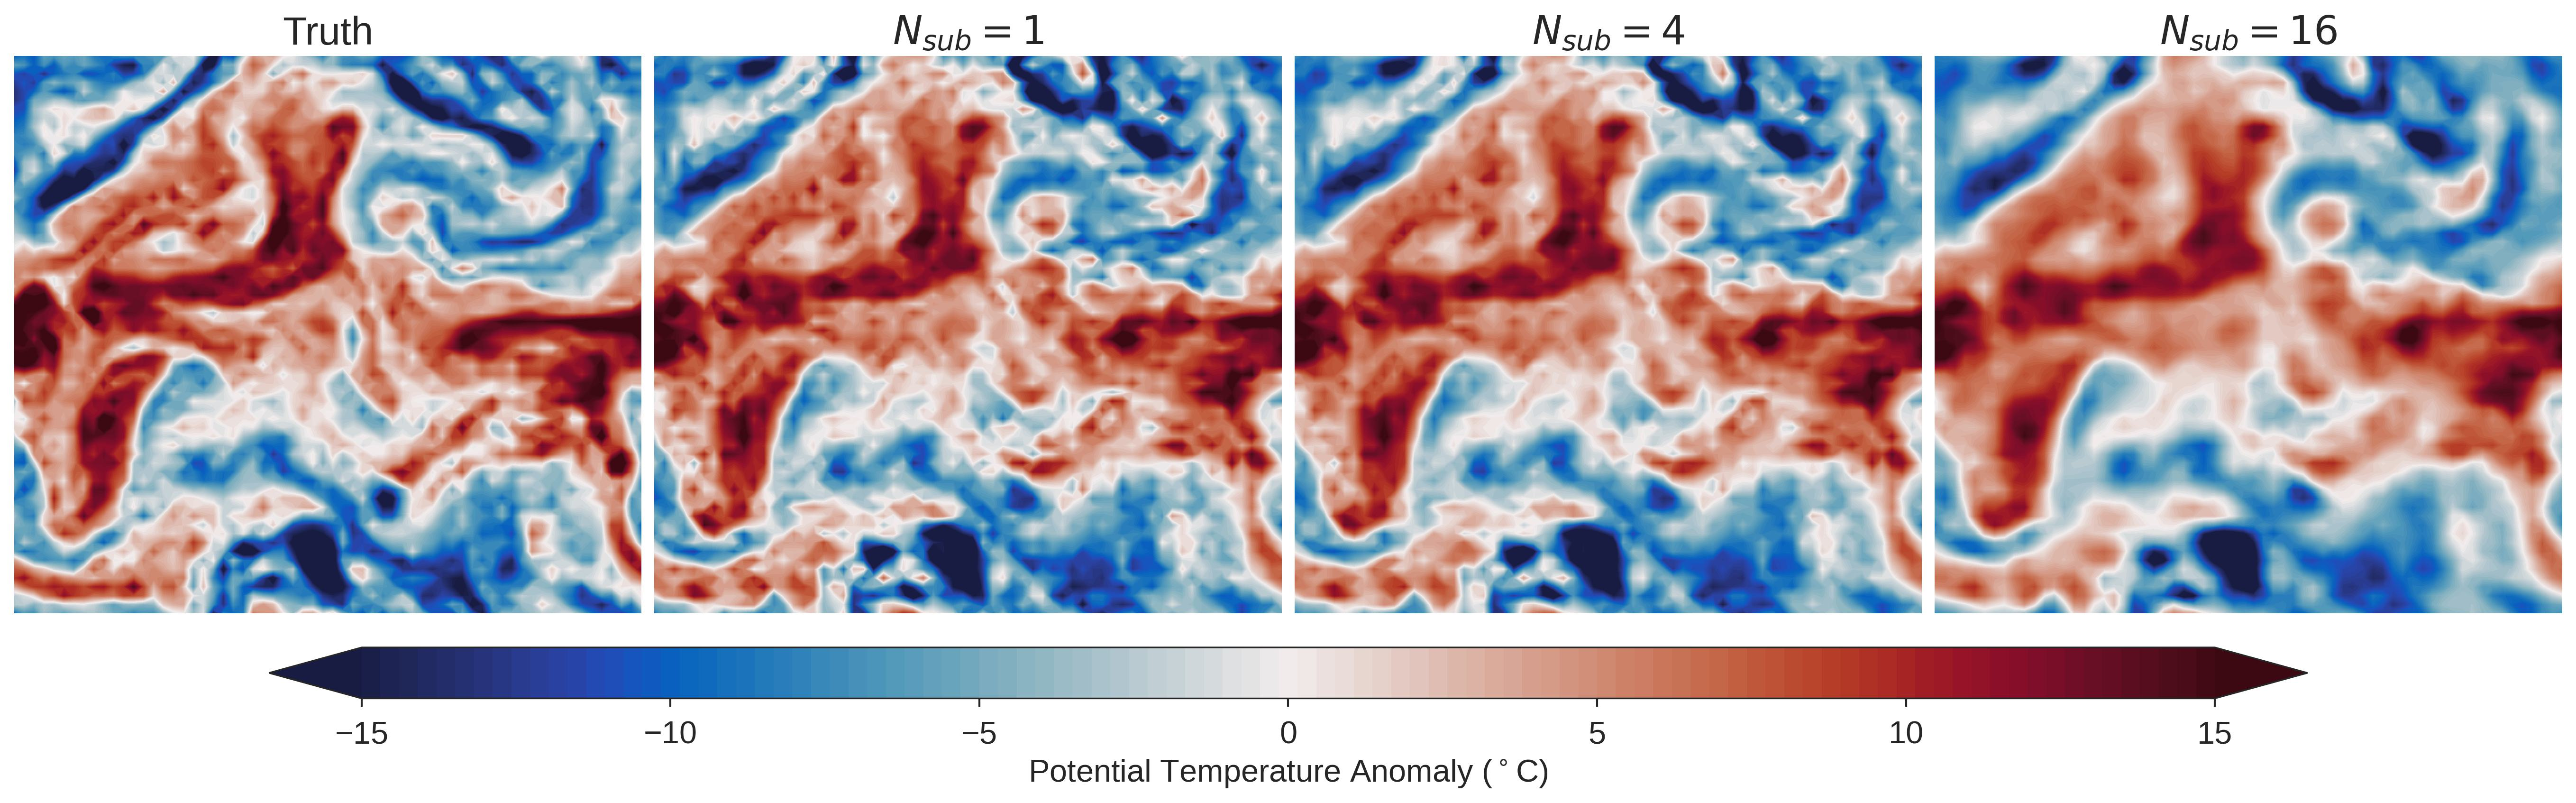
\includegraphics[width=\textwidth]{../figures/nvar_4hr_snap.jpg}
    \caption{One sample NVAR prediction from the test dataset for $\nsub =
        1,4,16$, shown in the second, third, and fourth rows at a lead time of 4~hours.
        The corresponding truth is shown in the far left panel.
        Here $\maxlag=1$ and only the surface level is shown.
    }
    \label{fig:nvar_qualitative}
\end{figure}

\begin{figure}
    \centering
    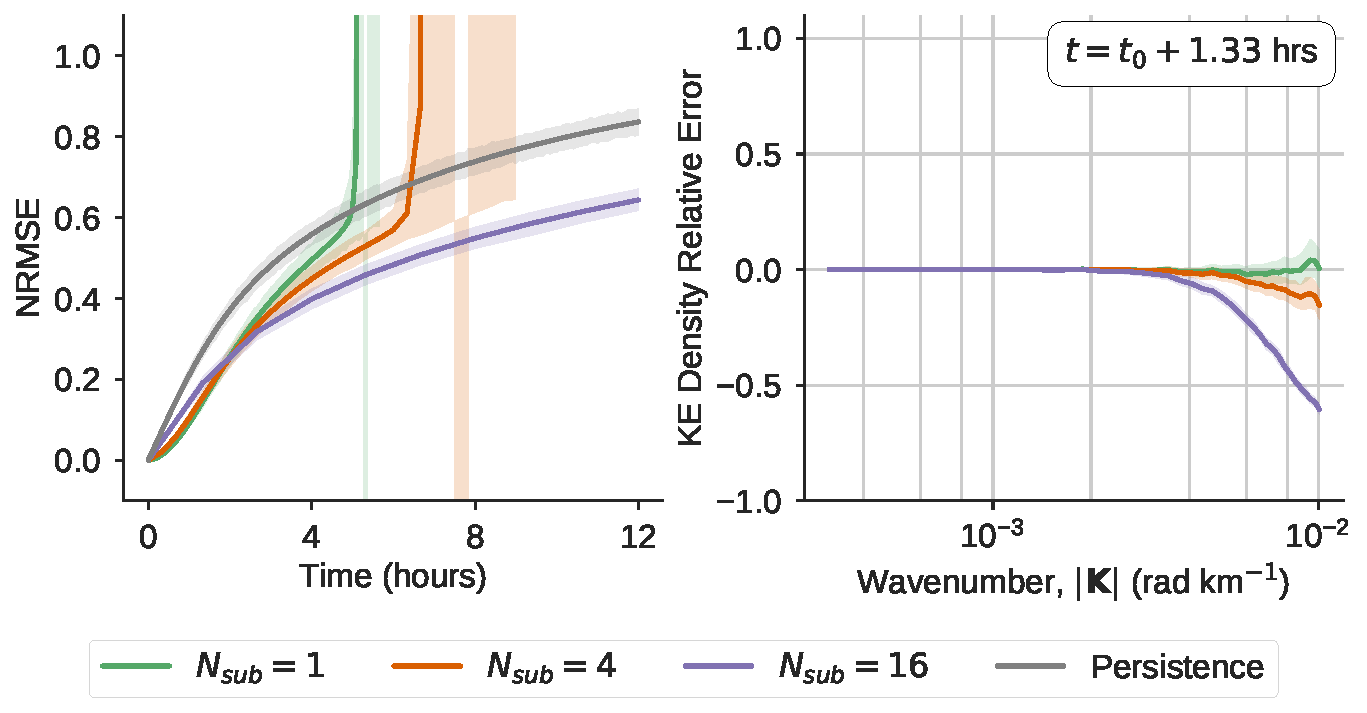
\includegraphics[width=.8\textwidth]{../figures/nvar-nrmse-and-kere.pdf}
    \caption{NRMSE (\cref{eq:nrmse}; left) and KE density
        relative error (\cref{eq:ke_relerr}; right)
        indicating prediction skill of the NVAR
        architecture using 50~samples from the test dataset.
        Solid lines indicate averages and shading indicates 99\% confidence
        interval.
        Here $\nlag=1$.
    }
    \label{fig:nvar_nrmse}
\end{figure}

% Describe the big plot
\cref{fig:nvar_qualitative} shows a qualitative comparison of NVAR predictions
as a function of $\nsub$, i.e., how frequently the training data are sampled and
the model makes predictions.
For this figure, we set $\nlag=1$, and note that both the NRMSE and a snapshot
of the KE density relative error corresponding to this configuration are shown in
\cref{fig:nvar_nrmse}.

At the model timestep ($\Delta \tau = \Delta t = 5$~min; $\nsub=1$), the NVAR predictions are
qualitatively similar to the truth for short forecast lead times.
That is, the NRMSE is near 0, and
many of the small scale features that exist in the truth are also evident
in the predictions.
However, at longer lead times the predictions become unstable.
NRMSE spikes rapidly at about 4~hours after numerical instabilities are
generated, which causes the NVAR model to produce physically unrealistic results.
For reference, \cref{fig:nvar_instabilities} shows a view of what these
numerical instabilities look like at their onset.
\todo{Do you think this figure is necessary?}

\begin{figure}
    \centering
    \begin{overpic}[width=.3\textwidth]{../figures/nvar_instabilities.jpg}
        \put(0, 0){\color{green}\linethickness{.2em}
            \polygon(43,52)(57,52)(57,39)(43,39)
        }
    \end{overpic}
    \caption{A view of the numerical instabilities generated by the NVAR model.
        The instabilities manifest as spiking oscillations, which are
        especially strong in the green box.
        This particular example occurs after 8~hours, given the same initial
        conditions in \cref{fig:nvar_qualitative} and $\nsub=1; \nlag=1$.
    }
    \label{fig:nvar_instabilities}
\end{figure}

As the temporal resolution of the data is reduced, i.e., as $\nsub$ increases,
the predictions are generally stable for a longer period of time.
\cref{fig:nvar_nrmse} shows that for $\nsub=4$, predictions are stable for roughly
6~hours, and for $\nsub=16$ no predictions generate numerical instabilities over the
12~hour window.
However, this stability comes with a cost: as the temporal resolution is
reduced, the model's representation of small scale features diminishes as these
features become more blurry or smoothed. This blurring effect is apparent in \cref{fig:nvar_qualitative}, where the prediction is qualitatively more blurry as $\nsub$ increases in each panel from left to right.

This smoothing behavior is captured quantitatively in the right panel of
\cref{fig:nvar_nrmse},
which shows the KE relative error as in \cref{eq:ke_nrmse}.
Here, we show the KE relative error after only 1.33~hours to show the behavior
before instabilities dominate the $\nsub=1$ predictions.
The plot indicates the degree of spectral bias in each solution, which is
largest at the smaller spatial scales, corresponding to higher wave numbers.

At $\nsub=1$ there is a small positive bias at the smallest resolved spatial
scales, indicating that this is when numerical instabilities are starting to
generate.
The subsampled runs, $\nsub=\{4,16\}$, show a negative bias, which corresponds
to a damped energy spectrum at the scales that are not resolved in the
qualitatively smooth predictions shown in \cref{fig:nvar_qualitative}.
This negative bias is clearly larger with higher subsampling, or reduced
temporal resolution.


\subsection{Prediction Skill as a Function of Memory}
\label{subsec:nvar-memory}

A key feature of RNNs and autoregressive models is that they retain memory of
previous system states.
Given the explicit nature of the NVAR architecture, we explore the effect of
adding memory by increasing $\nlag$, the number of lagged states used to create the
feature vector.
We first summarize how memory impacts prediction skill in
\cref{fig:nvar_nrmse_vs_lag}, which shows the NRMSE as a
function of $\nlag$ (colors) for each
subsampling factor $\nsub = \{1, 4, 16\}$ (panels).
For any value of $\nsub$, adding memory (increasing $\nlag$) reduces
the short term error.
However, adding memory also tends to increase error by the end of the forecast,
often leading to the development of numerical instabilities and an
incoherent solution.
Similarly, for any fixed value of $\nlag$, increasing the temporal resolution
(decreasing $\nsub$) shows the same behavior.

\begin{figure}
    \centering
    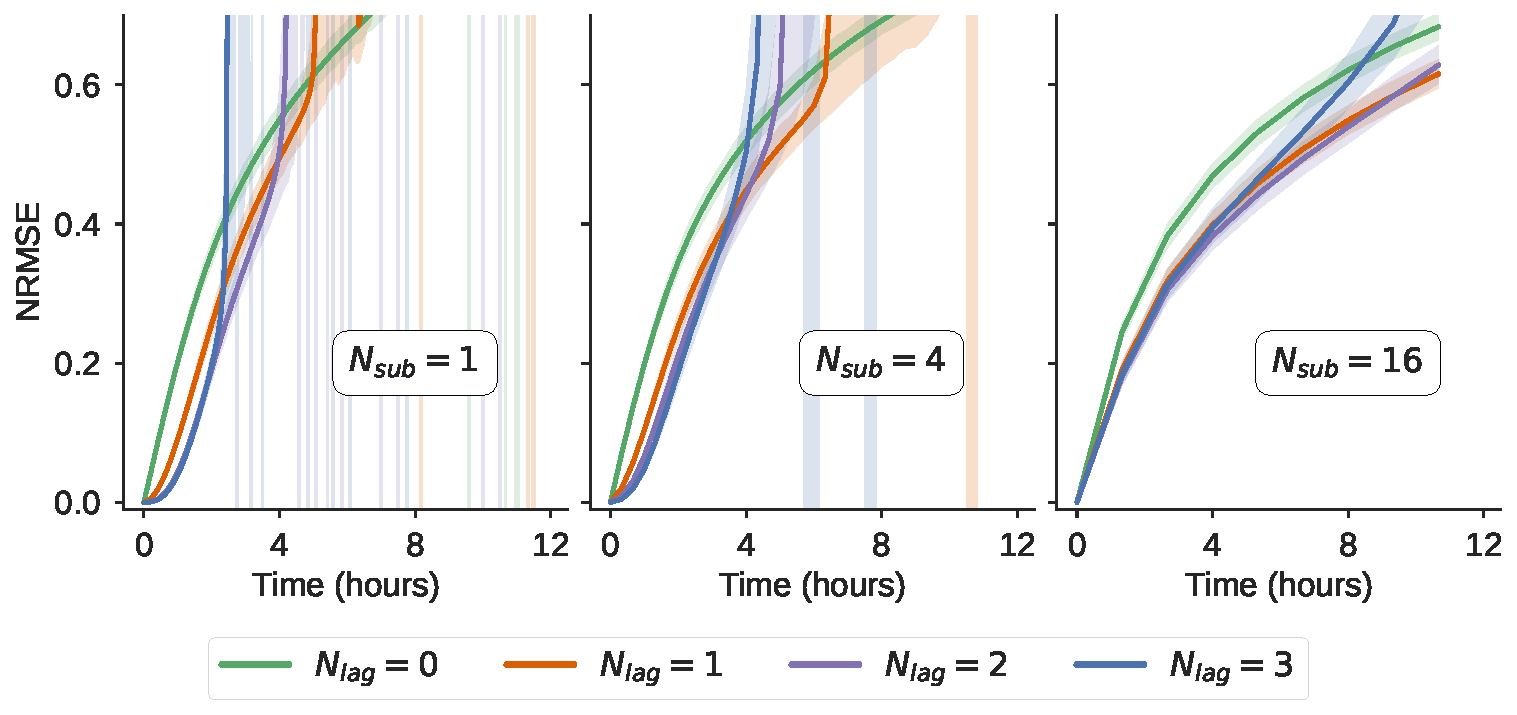
\includegraphics[width=\textwidth]{../figures/nvar_nrmse_vs_memory.pdf}
    \caption{NRMSE computed using NVAR at various temporal resolutions
        ($\nsub$; columns) and with variable memory capacities ($\nlag$;
        colors).
    }
    \label{fig:nvar_nrmse_vs_lag}
\end{figure}

To shed some light on how this additional memory impacts the solution,
we show the KE relative error
for the case of $\nsub=16$ as a function of time (panels) and $\nlag$ (colors)
in \cref{fig:nvar_ke_vs_lag}.
For about the first 4~hours, increasing memory improves prediction skill at all
spatial scales.
However, beyond this point, the overall NRMSE grows rapidly, the improvement
at small scales ($|\mathbf{K}|>4\cdot10^{-3}$~rad~km$^{-1}$) is more muted,
and error is propagated rapidly into the larger spatial scales.

We surmise that adding memory degrades the long term prediction skill because
the relationship between points further back in history are governed by higher
order nonlinear interactions that are incorrectly represented by
the simple local-quadratic relation that is used here.
As more terms are added that are incorrectly represented, the model becomes
more and more unstable.
The question is therefore how to retain the short term benefit of added memory
capacity throughout the forecast horizon while maintaining a stable trajectory.
While it may seem natural to explore higher order polynomials to
properly represent this history, we do not explore this further because the size
of the feature vector grows dramatically with the polynomial order
\citep{chen_next_2022}.
Another option would be to explore entirely different basis functions.
While this could be a potential option for future work, we note the findings of
\citet{zhang_catch-22_2022}, who show the extreme sensitivity of NVAR to the
form of nonlinearity imposed.
Given that it is an entirely open question on how to represent the smallest
scales of geophysical turbulence, we do not explore other basis functions, and
instead turn to the more general ESN architecture.

\begin{figure}
    \centering
    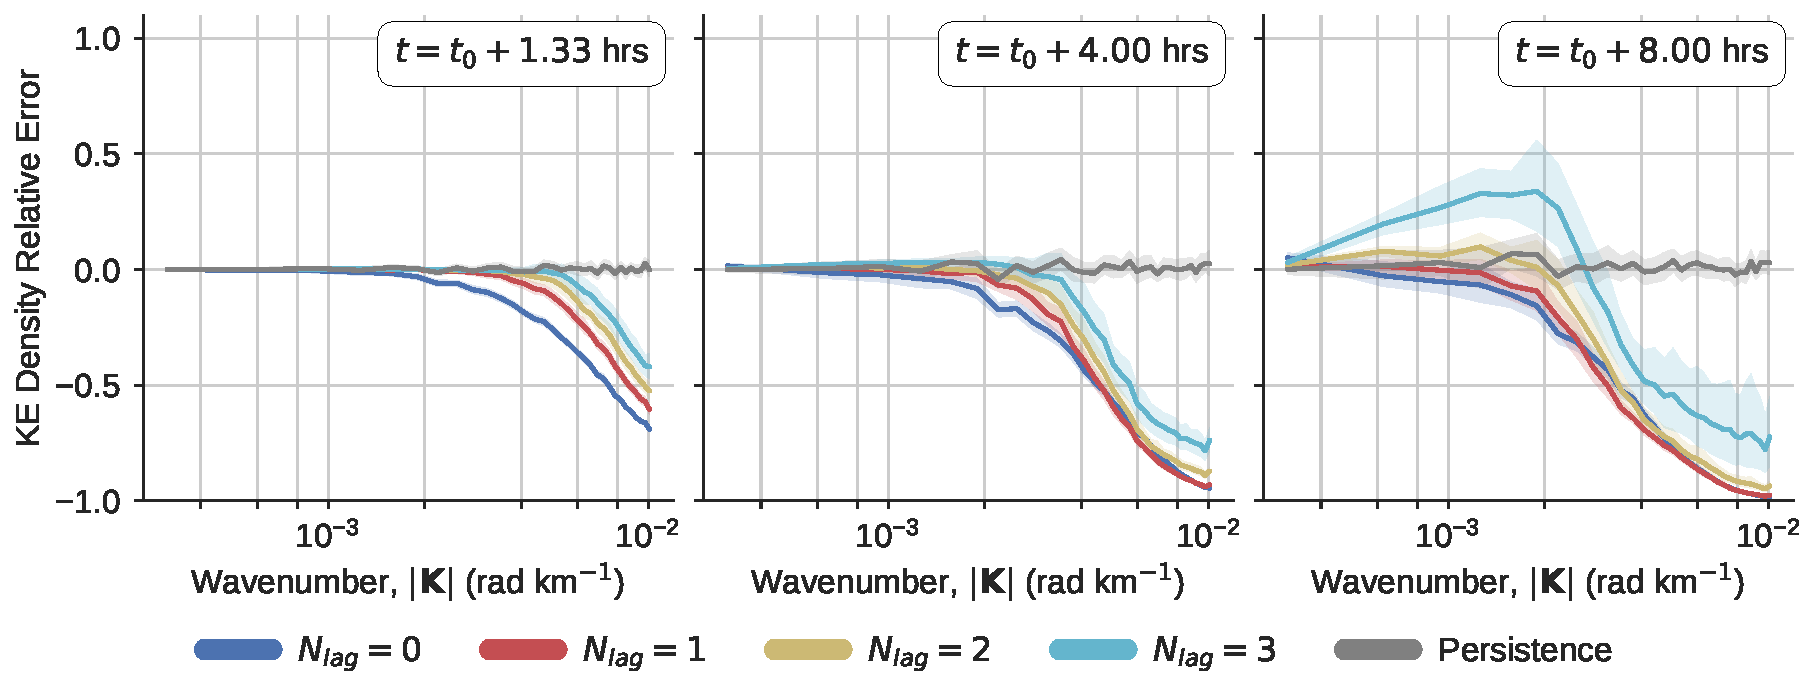
\includegraphics[width=\textwidth]{../figures/nvar_ke_relerr_vs_lag.pdf}
    \caption{Kinetic energy density relative error with $\nsub=16$ at various
        timesteps (columns) and memory capacity ($\nlag$; colors).
    }
    \label{fig:nvar_ke_vs_lag}
\end{figure}
